\section{Data collection and analysis}
In this section, we cover how we collected the data using the aforementioned program and we analyse the numerical results.
\subsection{Methodology}
Remembering the nature of the methods, which is qualitative, we established the following protocol for data collection:
\begin{enumerate}
    \item We fixed the following parameters:
          \begin{itemize}
              \item \textbf{number of boids} = 200, 500 and 1000;
              \item \textbf{field of view} = $290^{\circ}$;
              \item \textbf{range for the boids' initial positions} = $[-\frac{\text{number of boids}}{40}, \frac{\text{number of boids}}{40}]$;
              \item \textbf{number of timesteps analysed} = 500;
              \item \textbf{range of speed for the predator} = [3.0, 25.0];
              \item \textbf{maximum change in speed for the predator} = 1.5;
              \item \textbf{attraction parameter for the predator} = 2.0;
          \end{itemize}
    \item We performed, for every method and for the three numbers of boids listed, manual tuning of the free parameters by testing their qualitative output, which was in turn checked by producing a video or a gif of the duration of 500 timesteps;
    \item After finding the adequate parameters, we collected the correlation function and the polarization over time for the flock when free, attacked by a predator and approaching an obstacle, be it a wall or a column.
\end{enumerate}
\subsection{Reynolds' method: results and comments}
\subsubsection{Results}
The results below were obtained by employing the parameters listed in \autoref{tab:reynolds_params}. \\
\begin{table}[ht]
    \centering
    \begin{tabular}{|c|c|c|c|}
        \hline
        \textbf{Parameter}    & \textbf{200}   & \textbf{500}   & \textbf{1000}  \\
                              & \textbf{boids} & \textbf{boids} & \textbf{boids} \\ \hline
        Cohesion              & 5.5            & 5.5            & 5.5            \\ \hline
        Alignment             & 0.050          & 0.20           & 0.80           \\ \hline
        Separation            & 0.025          & 0.10           & 0.50           \\ \hline
        Action range          & 20             & 20             & 20             \\ \hline
        Speed range           & 1.0-4.0        & 1.0-4.0        & 1.0-4.0        \\ \hline
        Maximum delta         & 0.25           & 0.25           & 0.25           \\ \hline
        Predator action range & 40             & 40             & 60             \\ \hline
        Predator separation   & 0.60           & 5              & 5              \\ \hline
        Column action range   & 5              & 10             & 10             \\ \hline
        Column separation     & 0.07           & 0.125          & 0.12           \\ \hline
        Wall action range     & 30             & 35             & 35             \\ \hline
        Wall separation       & 0.005          & 0.0045         &
        0.0045                                                                   \\ \hline\end{tabular}
    \caption{Parameters found by manual tuning for Reynolds' model.}
    \label{tab:reynolds_params}
\end{table}
Reynolds' model proved itself to be, as far as quantitative analysis go, not predictable and rather sensitive to the initial conditions (which are the only random variable of the method). As expected, polarization stayed stably close to one, with the necessary oscillations deriving from the situations (for example, when hitting a wall it briefly decreased); such results can be inspected regarding the 1000 boids flock in \autoref{fig:pol_reynolds}, but are consistent regardless of the number of boids. \\
\begin{figure}[ht]
    \centering
    \begin{subfigure}{0.95\linewidth}
        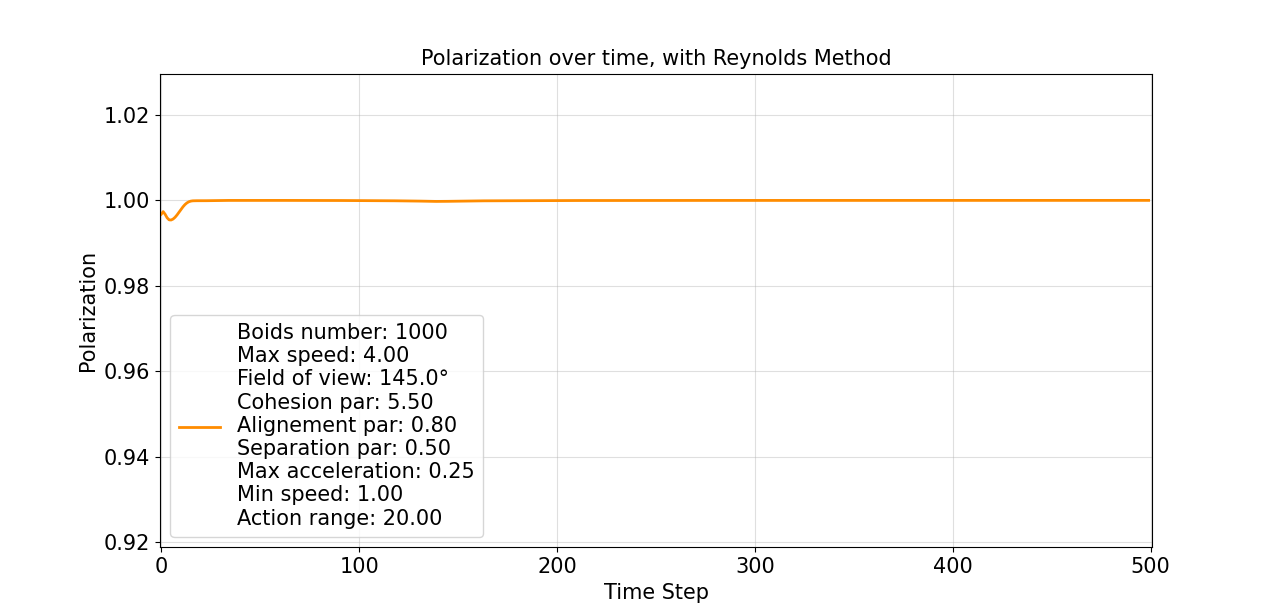
\includegraphics[width=\linewidth]{pictures/sec_4/reynolds/p_1000_free.png}
        \subcaption{Polarization over time for a free flock of 1000 boids.}
    \end{subfigure}
    \begin{subfigure}{0.95\linewidth}
        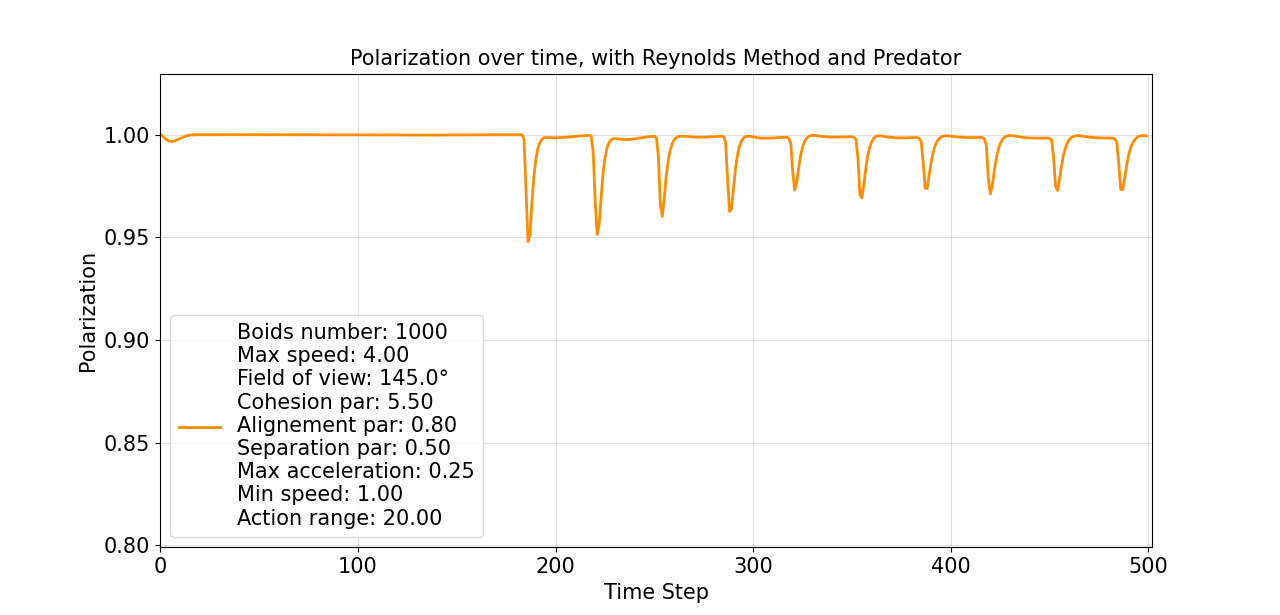
\includegraphics[width=\linewidth]{pictures/sec_4/reynolds/p_1000_pred.png}
        \subcaption{Polarization over time for a flock of 1000 boids while attacked by a predator.}
    \end{subfigure}
    \begin{subfigure}{0.95\linewidth}
        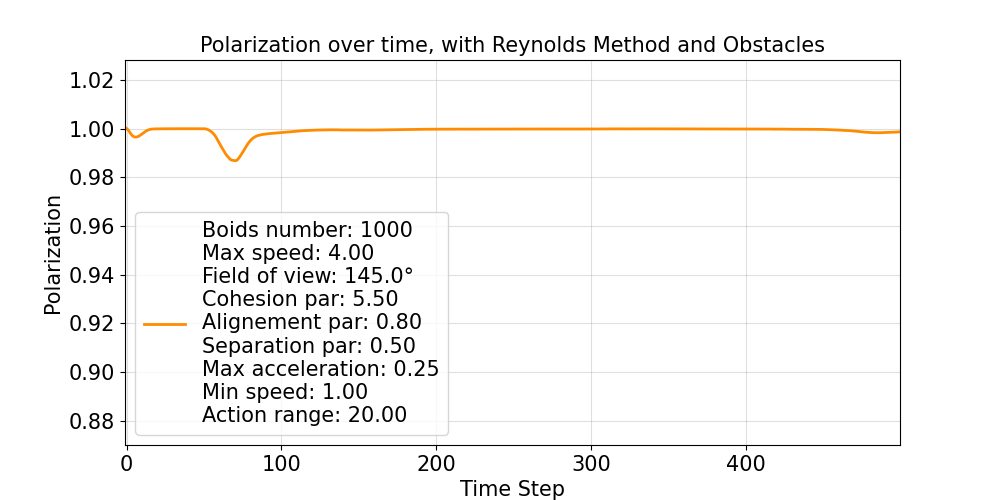
\includegraphics[width=\linewidth]{pictures/sec_4/reynolds/p_1000_column.png}
        \subcaption{Polarization over time for a flock of 1000 boids reacting to a column.}
    \end{subfigure}
    \begin{subfigure}{0.95\linewidth}
        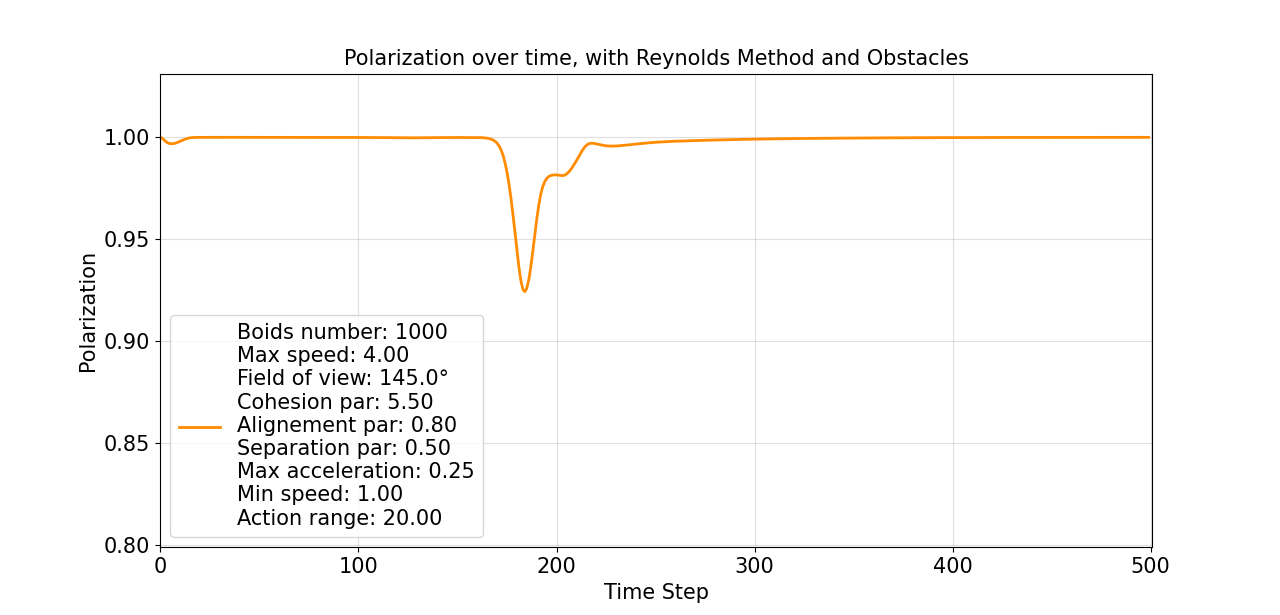
\includegraphics[width=\linewidth]{pictures/sec_4/reynolds/p_1000_wall.png}
        \subcaption{Polarization over time for a flock of 1000 boids reacting to a wall.}
    \end{subfigure}
    \caption{Polarization over time plotted in different situations for a flock simulated using Reynolds' model.}
    \label{fig:pol_reynolds}
\end{figure}
The same cannot be said regarding the correlation function. Although in our analysis we did find some that exhibited the already explained two dominion behaviour, they were not the norm; in general, the typical correlation function was more akin to a random oscillation around 0, as shown in \autoref{fig:reynolds_cr}. \\
\begin{figure}[ht]
    \centering
    \begin{subfigure}{0.95\linewidth}
        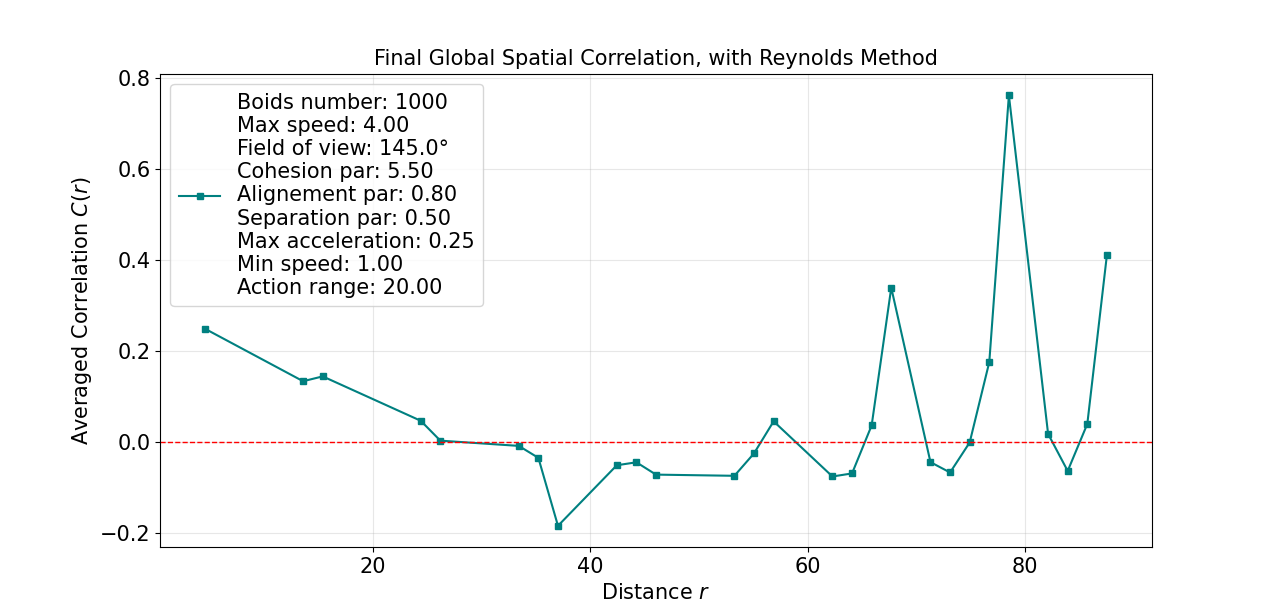
\includegraphics[width=\linewidth]{pictures/sec_4/reynolds/cr_1000_free.png}
        \subcaption{Correlation function of a 1000 boids free flock.}
    \end{subfigure}
    \begin{subfigure}{0.95\linewidth}
        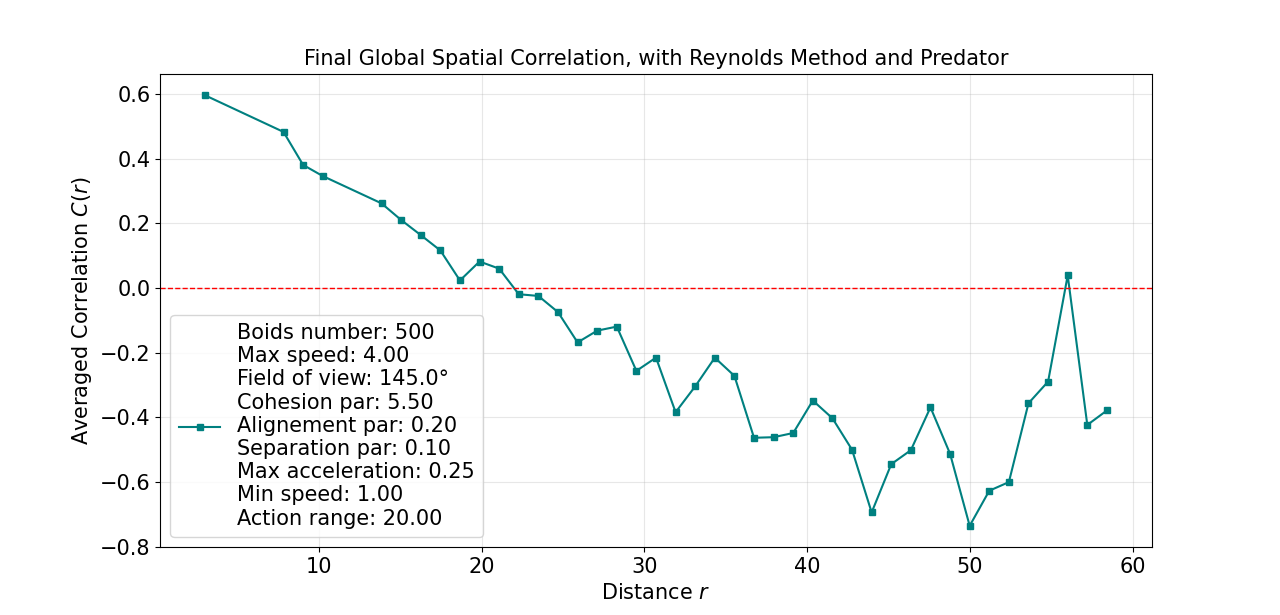
\includegraphics[width=\linewidth]{pictures/sec_4/reynolds/cr_500_pred.png}
        \subcaption{Correlation function of a 500 boids flock attacked by a predator.}
    \end{subfigure}
    \begin{subfigure}{0.95\linewidth}
        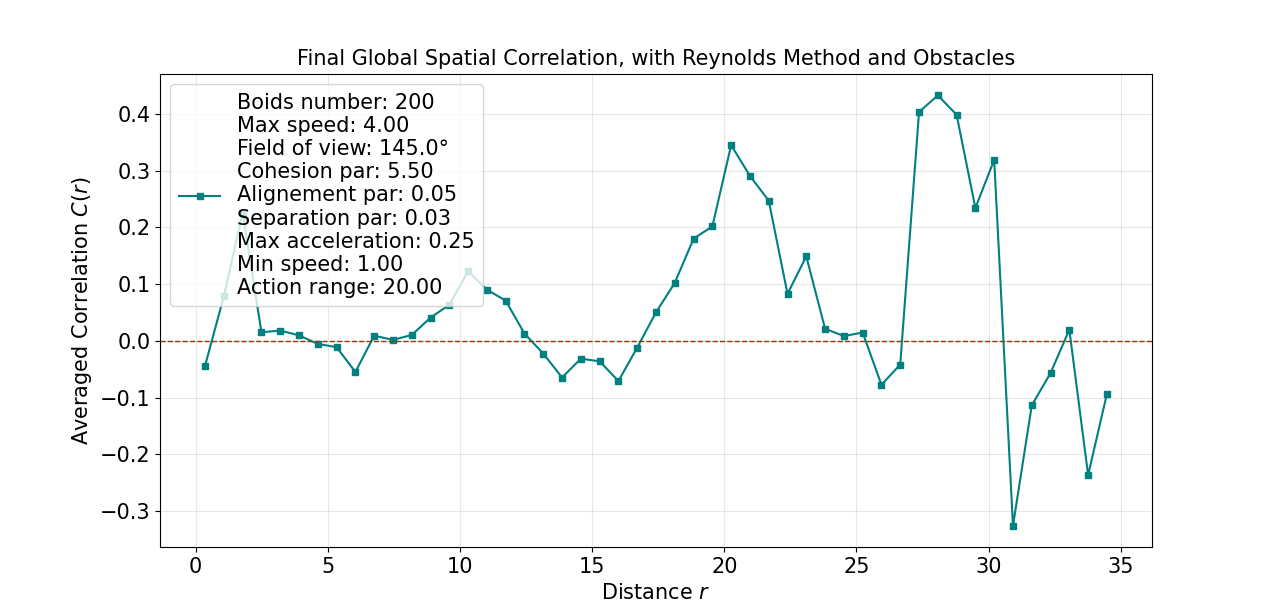
\includegraphics[width=\linewidth]{pictures/sec_4/reynolds/cr_200_column.png}
        \subcaption{Correlation function of a 200 boids flock reacting to a column.}
    \end{subfigure}
    \begin{subfigure}{0.95\linewidth}
        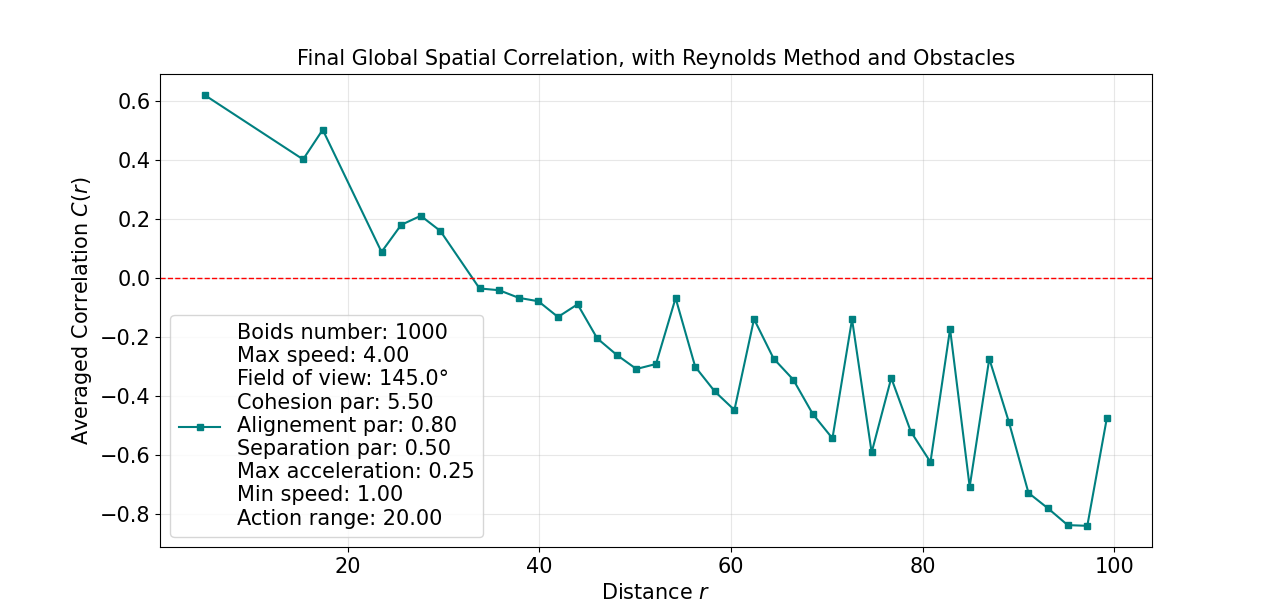
\includegraphics[width=\linewidth]{pictures/sec_4/reynolds/cr_1000_wall.png}
        \subcaption{Correlation function of a 1000 boids flock reacting to a wall.}
    \end{subfigure}
    \caption{Correlation functions plotted in different situations for a flock simulated using Reynolds' model.}
    \label{fig:reynolds_cr}
\end{figure}
\subsubsection{Comments}
While manually tuning the model, we noticed how sensitive Reynolds' model is to the initial parameters, and how unsuited for quantitative analysis it is, since the correlation function tends to be unstable over different iterations of the model. It is also, as stated before, remarkably sensitive to the initial conditions.
\subsection{Vicsek's method: results and comments}
\subsubsection{Results}
The following results were obtained by employing the parameters listed in \autoref{tab:vicsek_params}.
\begin{table}[ht]
    \centering
    \begin{tabular}{|c|c|c|c|}
        \hline
        \textbf{Parameter} & \textbf{200}   & \textbf{500}   & \textbf{1000}  \\
                           & \textbf{boids} & \textbf{boids} & \textbf{boids} \\ \hline
        Speed              & 2.0            & 2.0            & 2.0            \\ \hline
        Action range       & 10             & 20             & 30             \\ \hline
        Angular noise      & $1.0^\circ$    & $1.0^\circ$    & $1.0^\circ$    \\ \hline
    \end{tabular}
    \caption{Parameters found by manual tuning for Vicsek' model.}
    \label{tab:vicsek_params}
\end{table}
As was predictable, Vicsek's model, qualitatively, does not perform well. It obtains reasonably acceptable (albeit very artificial looking) simulations for free and wall-approaching flocks, but when attacked by a predator or approaching a column the flock does not behave correctly, and gets split. \\
Quantitatively speaking, the polarization function is predictably close to one (the model concerns only velocity alignment, after all). \\
\begin{figure}
    \centering
    \begin{subfigure}{0.95\linewidth}
        
\includegraphics[width=\linewidth]{pictures/sec_4/vicsek/200_boids_vicsek/free_pol_fun.png}
        \subcaption{Polarization over time of a 200 boids free flock.}
    \end{subfigure}
    \begin{subfigure}{0.95\linewidth}
        
\includegraphics[width=\linewidth]{pictures/sec_4/vicsek/500_boids_vicsek/predator_pol_fun.png}
        \subcaption{Polarization over time of a 500 boids flock while attacked by a predator.}
    \end{subfigure}
    \begin{subfigure}{0.95\linewidth}
        
\includegraphics[width=\linewidth]{pictures/sec_4/vicsek/1000_boids_vicsek/column_pol_fun.png}
        \subcaption{Polarization over time of a 1000 boids flock reacting to a column.}
    \end{subfigure}
    \begin{subfigure}{0.95\linewidth}
        
\includegraphics[width=\linewidth]{pictures/sec_4/vicsek/200_boids_vicsek/wall_pol_fun.png}
        \subcaption{Polarization over time of a 2000 boids flock reacting to a wall.}
    \end{subfigure}
    \caption{Polarization over time plotted in different situations for a flock simulated using Vicsek's model.}
    \label{fig:vicsek_pol}
\end{figure}
The correlation function exhibits the correct behaviour both in the case of a flock attacked by a predator and reacting to a column, as seen in \autoref{fig:vicsek_cr}, but this results have to be paired with the bad qualitative output.
\begin{figure}
    \centering
    \begin{subfigure}{0.95\linewidth}
        
\includegraphics[width=\linewidth]{pictures/sec_4/vicsek/200_boids_vicsek/free_cor_fun.png}
        \subcaption{Correlation function of a 200 boids free flock.}
    \end{subfigure}
    \begin{subfigure}{0.95\linewidth}
        
\includegraphics[width=\linewidth]{pictures/sec_4/vicsek/500_boids_vicsek/predator_cor_fun.png}
        \subcaption{Correlation function of a 500 boids flock while attacked by a predator.}
    \end{subfigure}
    \begin{subfigure}{0.95\linewidth}
        
\includegraphics[width=\linewidth]{pictures/sec_4/vicsek/1000_boids_vicsek/column_cor_fun.png}
        \subcaption{Correlation function of a 1000 boids flock reacting to a column.}
    \end{subfigure}
    \begin{subfigure}{0.95\linewidth}
        
\includegraphics[width=\linewidth]{pictures/sec_4/vicsek/200_boids_vicsek/wall_cor_fun.png}
        \subcaption{Correlation function of a 2000 boids flock reacting to a wall.}
    \end{subfigure}
    \caption{Correlation functions plotted in different situations for a flock simulated using Vicsek's model.}
    \label{fig:vicsek_cr}
\end{figure}
\subsubsection{Comments}
Vicsek's mode, while less sensitive to parameters than Reynolds', has its own share of problems, both quantitative and qualitative. The most important ones are the latter, since Vicsek's model, as stated before, is not fit for this type of analysis. Quantitatively, its problems lay in the fact that, while polarization exhibits good results (apart form the case of a predator attacking the flock), the correlation function only exhibits the correct behaviour in two of the four analysed scenarios, which are also the ones in which the model qualitatively performs worse.
\subsection{Couzin's method: results and comments}
\subsubsection{Results}
The following results were obtained by employing the parameters listed in \autoref{tab:couzin_params}.
\begin{table}[ht]
    \centering
    \begin{tabular}{|c|c|c|c|}
        \hline
        \textbf{Parameter} & \textbf{200}   & \textbf{500}   & \textbf{1000}  \\
                           & \textbf{boids} & \textbf{boids} & \textbf{boids} \\ \hline
        Speed              & 2.0            & 2.0            & 2.0            \\ \hline
        ZOA                & 20             & 25             & 40$^*$         \\ \hline
        ZOO                & 10             & 20             & 25             \\ \hline
        ZOR                & 1              & 1.5            & 3              \\ \hline
        Maximum steering   & $1.0^\circ$    & $1.0^\circ$    & $1.0^\circ$    \\ \hline
        angle (free)       &                &                &                \\ \hline
        Maximum steering   & $5.0^\circ$    & $7.5^\circ$    & $5.0^\circ$    \\ \hline
        angle (predator)   &                &                &                \\ \hline
        Maximum steering   & $3.0^\circ$    & $1.0^\circ$    & $1.0^\circ$    \\ \hline
        angle (column)     &                &                &                \\ \hline
        Maximum steering   & $3.0^\circ$    & $3.5^\circ$    & $3.0^\circ$    \\ \hline
        angle (wall)       &                &                &                \\ \hline
        Angular noise      & $0.1^\circ$    & $0.1^\circ$    & $0.1^\circ$    \\ \hline
    \end{tabular}
    \caption{Parameters found by manual tuning for Couzin's model. \\
        $^*$For the 1000 boids simulation regarding the reaction to a column, the ZOA was set to 35.}
    \label{tab:couzin_params}
\end{table}
Couzin's model, although more sentitive to the parameters than the other (as the reader may infer from the tables), is the one that both qualitatively and quantitatively performs best. As for the other methods, polarization is stably close to one, with the necessary oscillations deriving from the situations; such results can be inspected regarding the 1000 boids flock in \autoref{fig:pol_couzin}, but are consistent regardless of the number of boids. \\
\begin{figure}[ht]
    \centering
    \begin{subfigure}{0.95\linewidth}
        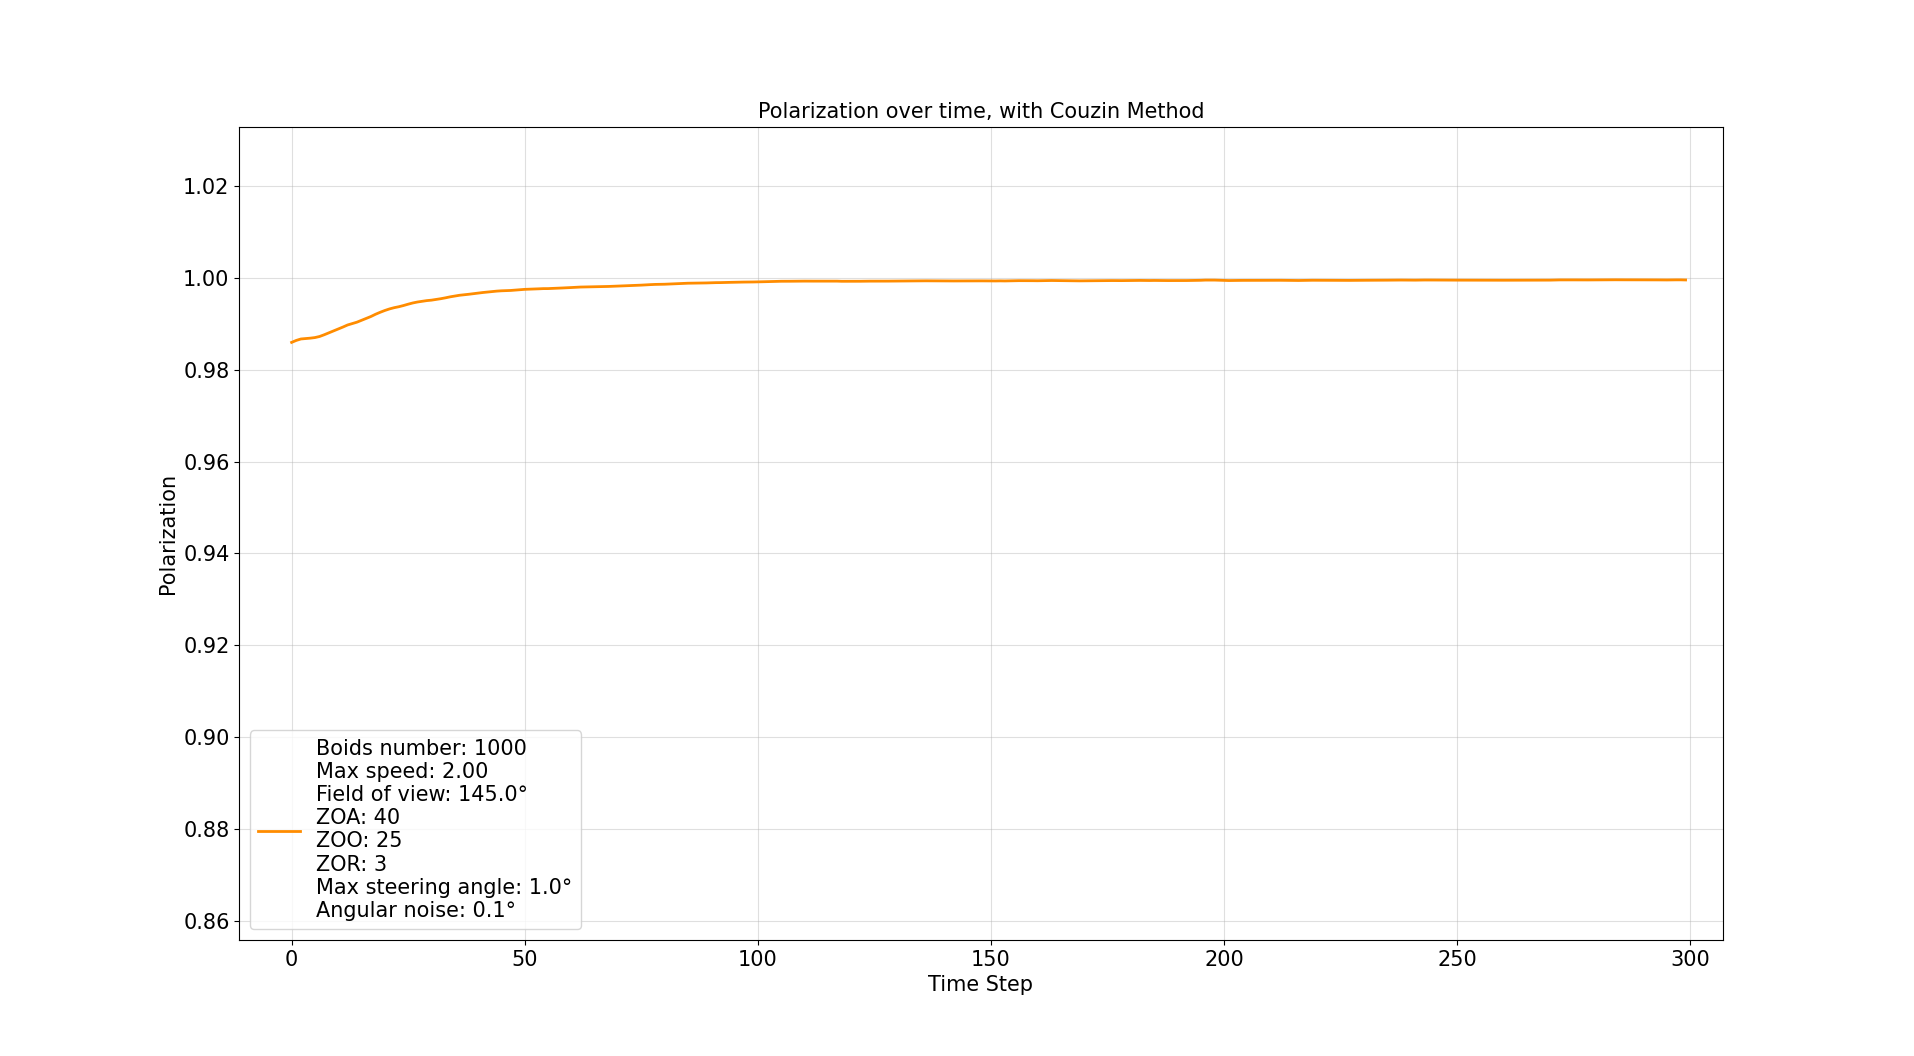
\includegraphics[width=\linewidth]{pictures/sec_4/couzin/1000_boids_couzin/free_pol_fun.png}
        \subcaption{Polarization over time for a free flock of 1000 boids.}
    \end{subfigure}
    \begin{subfigure}{0.95\linewidth}
        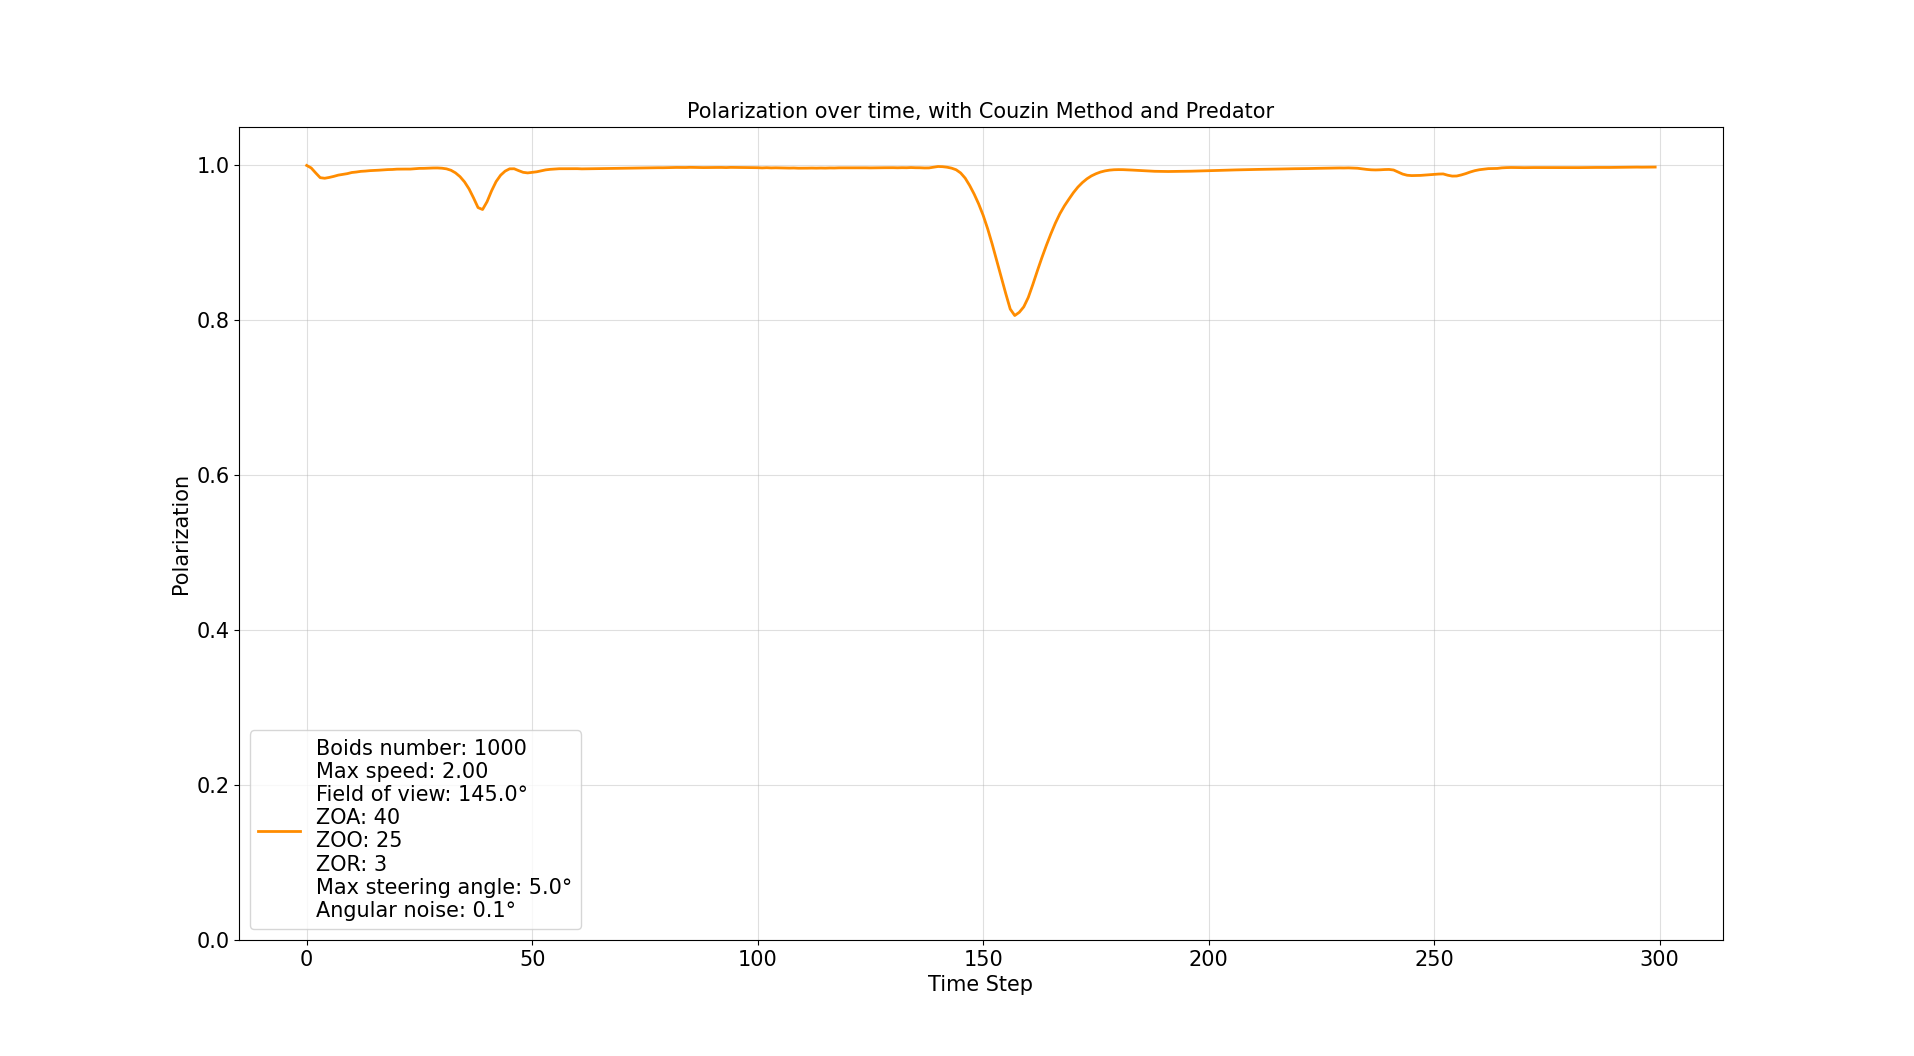
\includegraphics[width=\linewidth]{pictures/sec_4/couzin/1000_boids_couzin/predator_pol_fun.png}
        \subcaption{Polarization over time for a flock of 1000 boids while attacked by a predator.}
    \end{subfigure}
    \begin{subfigure}{0.95\linewidth}
        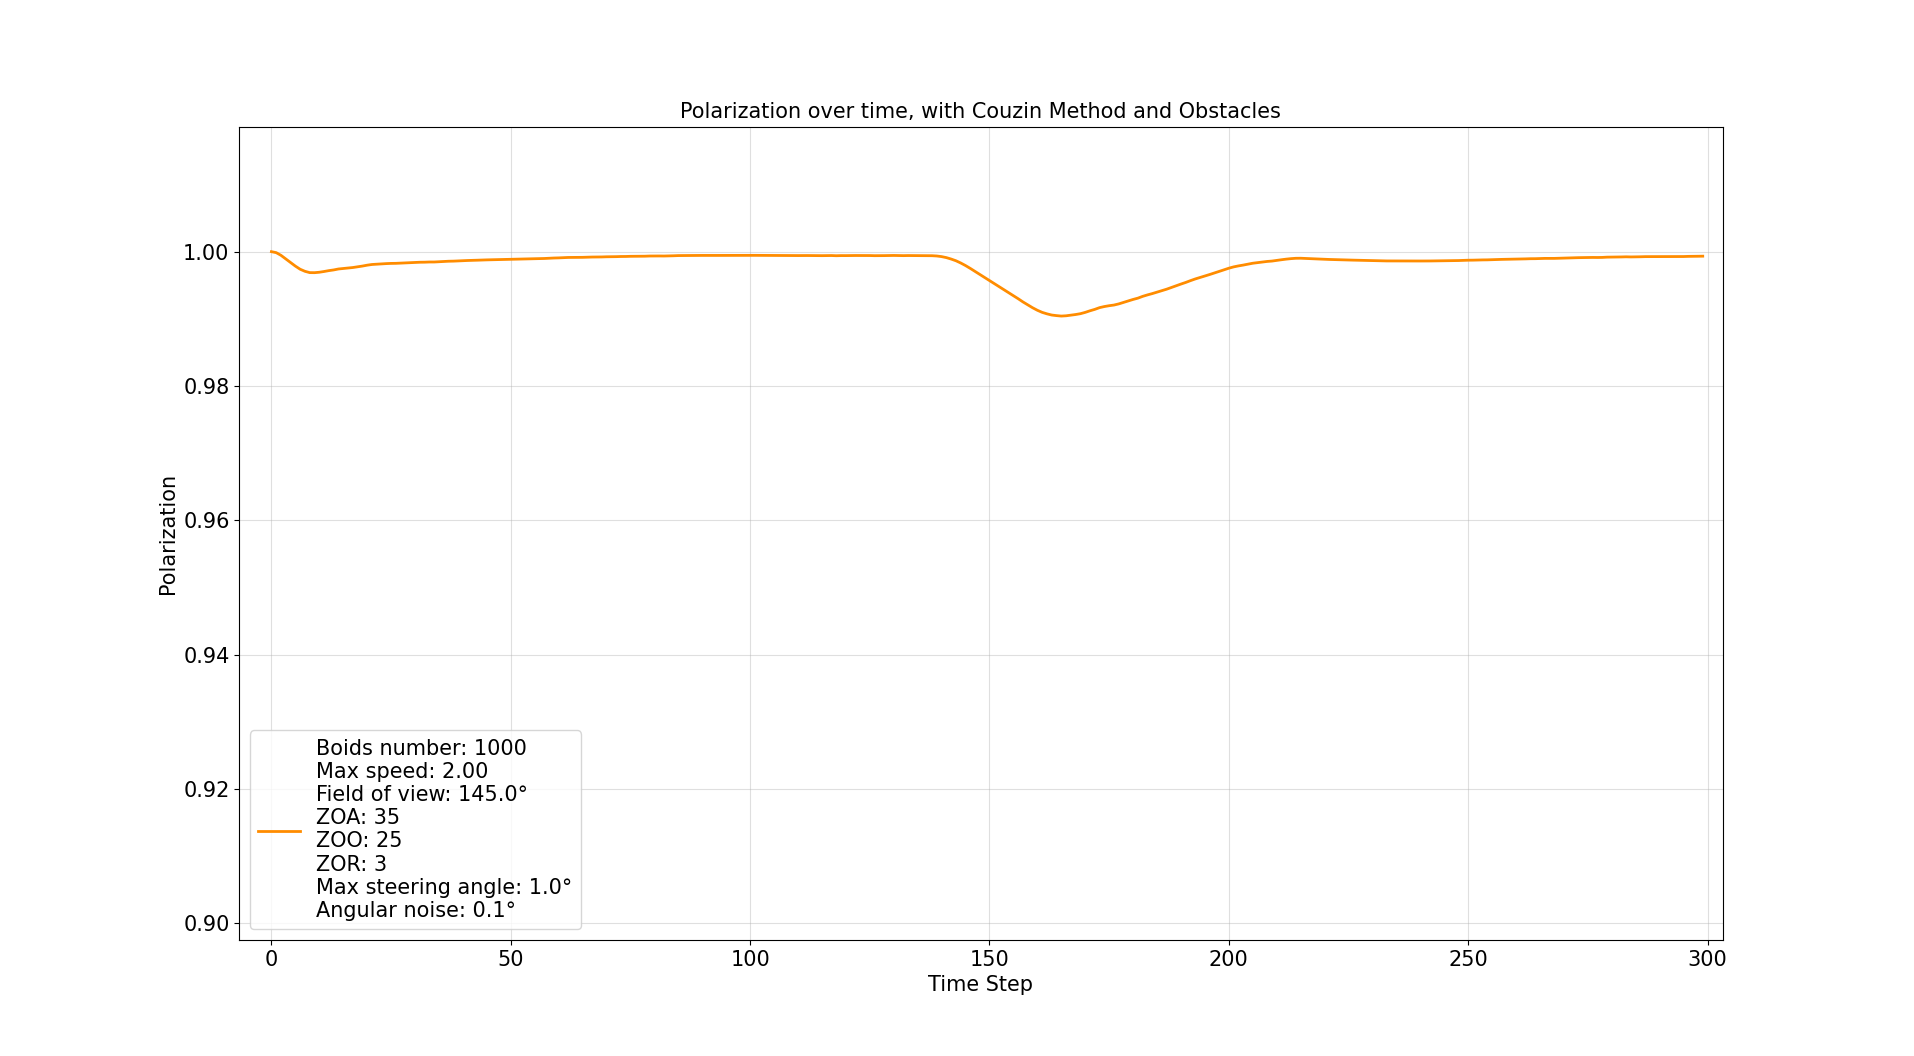
\includegraphics[width=\linewidth]{pictures/sec_4/couzin/1000_boids_couzin/column_pol_fun.png}
        \subcaption{Polarization over time for a flock of 1000 boids reacting to a column.}
    \end{subfigure}
    \begin{subfigure}{0.95\linewidth}
        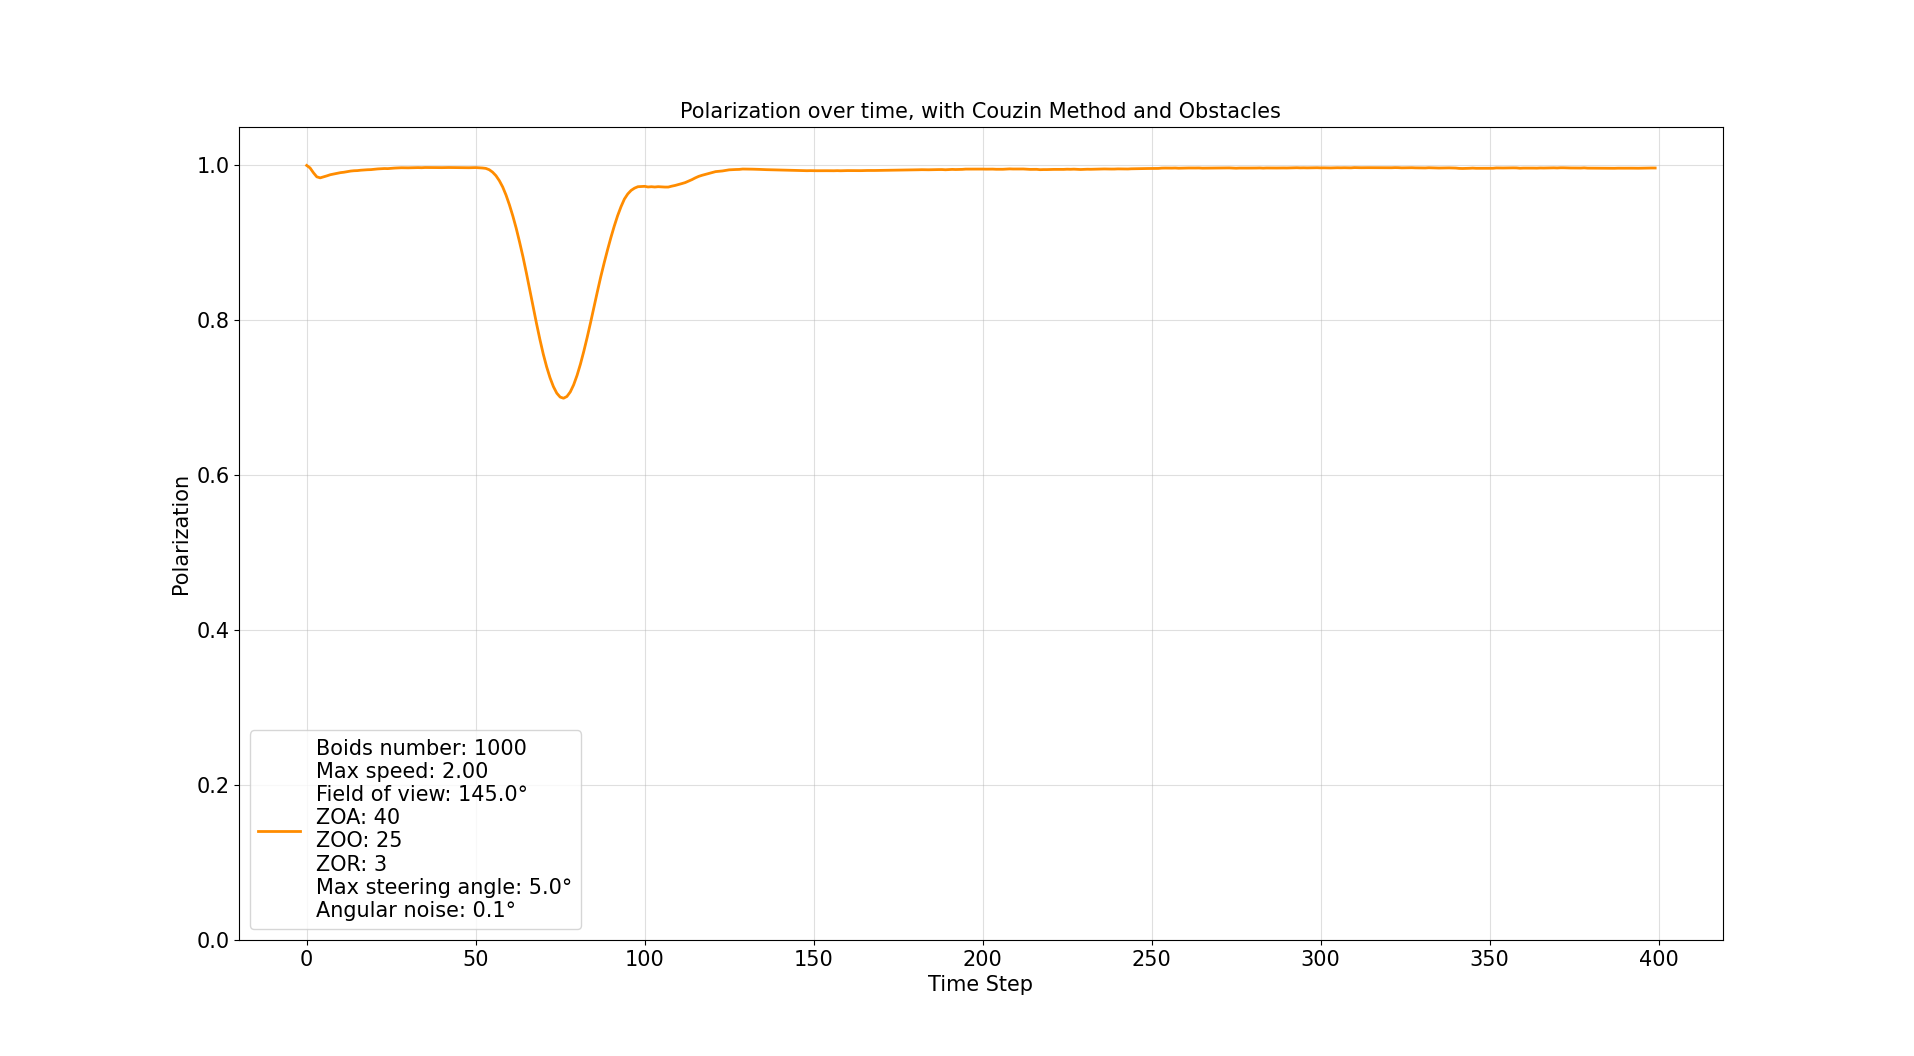
\includegraphics[width=\linewidth]{pictures/sec_4/couzin/1000_boids_couzin/wall_pol_fun.png}
        \subcaption{Polarization over time for a flock of 1000 boids reacting to a wall.}
    \end{subfigure}
    \caption{Polarization over time plotted in different situations for a flock simulated using Couzin's model.}
    \label{fig:pol_couzin}
\end{figure}
The correlation function, as shown in \autoref{fig:couzin_cr}, performs well in all of the analyzed scenarios but one, namely the one with the predator; the reader should be made aware that for the 1000 boids flock the correlation function did actually exhibit the already explained two-domain behaviour, but the pattern of starting to grow after a certain distance was consistent with the other simulations.
\begin{figure}
    \centering
    \begin{subfigure}{0.95\linewidth}
        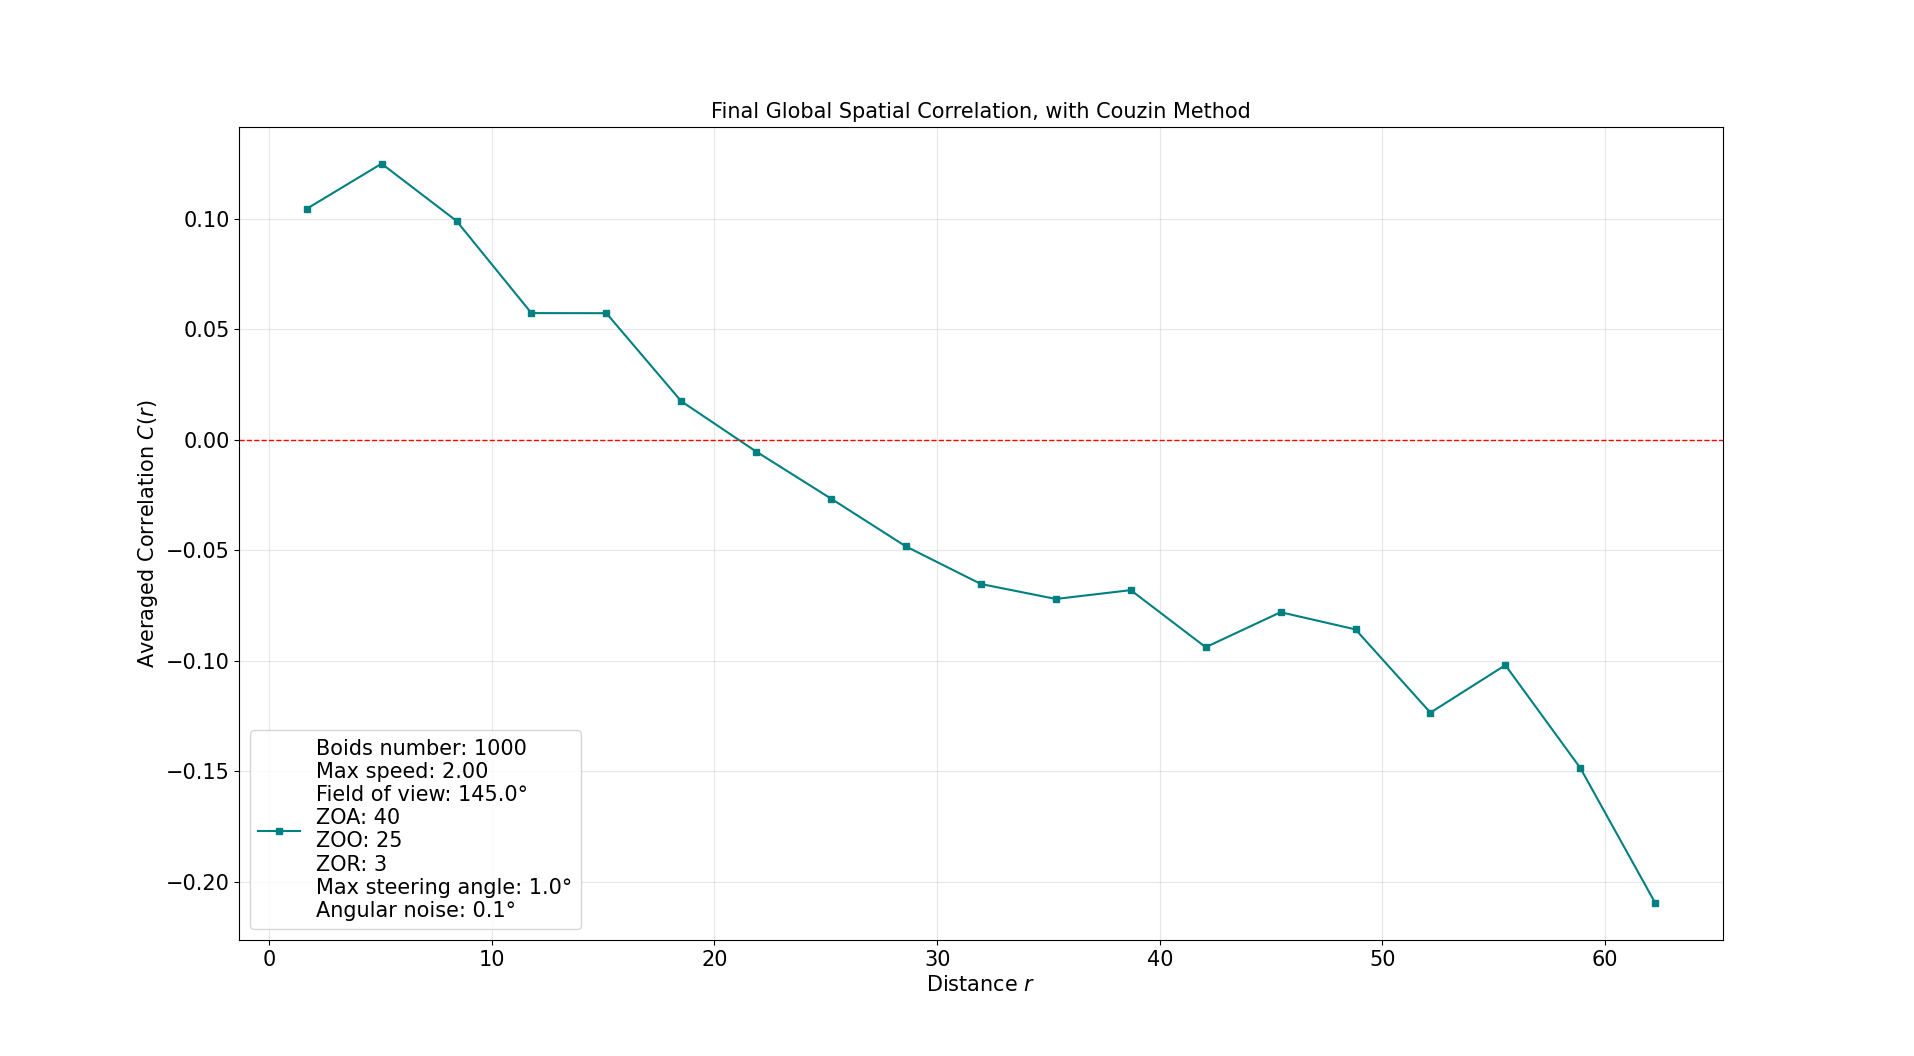
\includegraphics[width=\linewidth]{pictures/sec_4/couzin/1000_boids_couzin/free_cor_fun.png}
        \subcaption{Correlation function of a 1000 boids free flock.}
    \end{subfigure}
    \begin{subfigure}{0.95\linewidth}
        
\includegraphics[width=\linewidth]{pictures/sec_4/couzin/200_boids_couzin/predator_cor_fun.png}
        \subcaption{Correlation function of a 200 boids flock while attacked by a predator.}
    \end{subfigure}
    \begin{subfigure}{0.95\linewidth}
        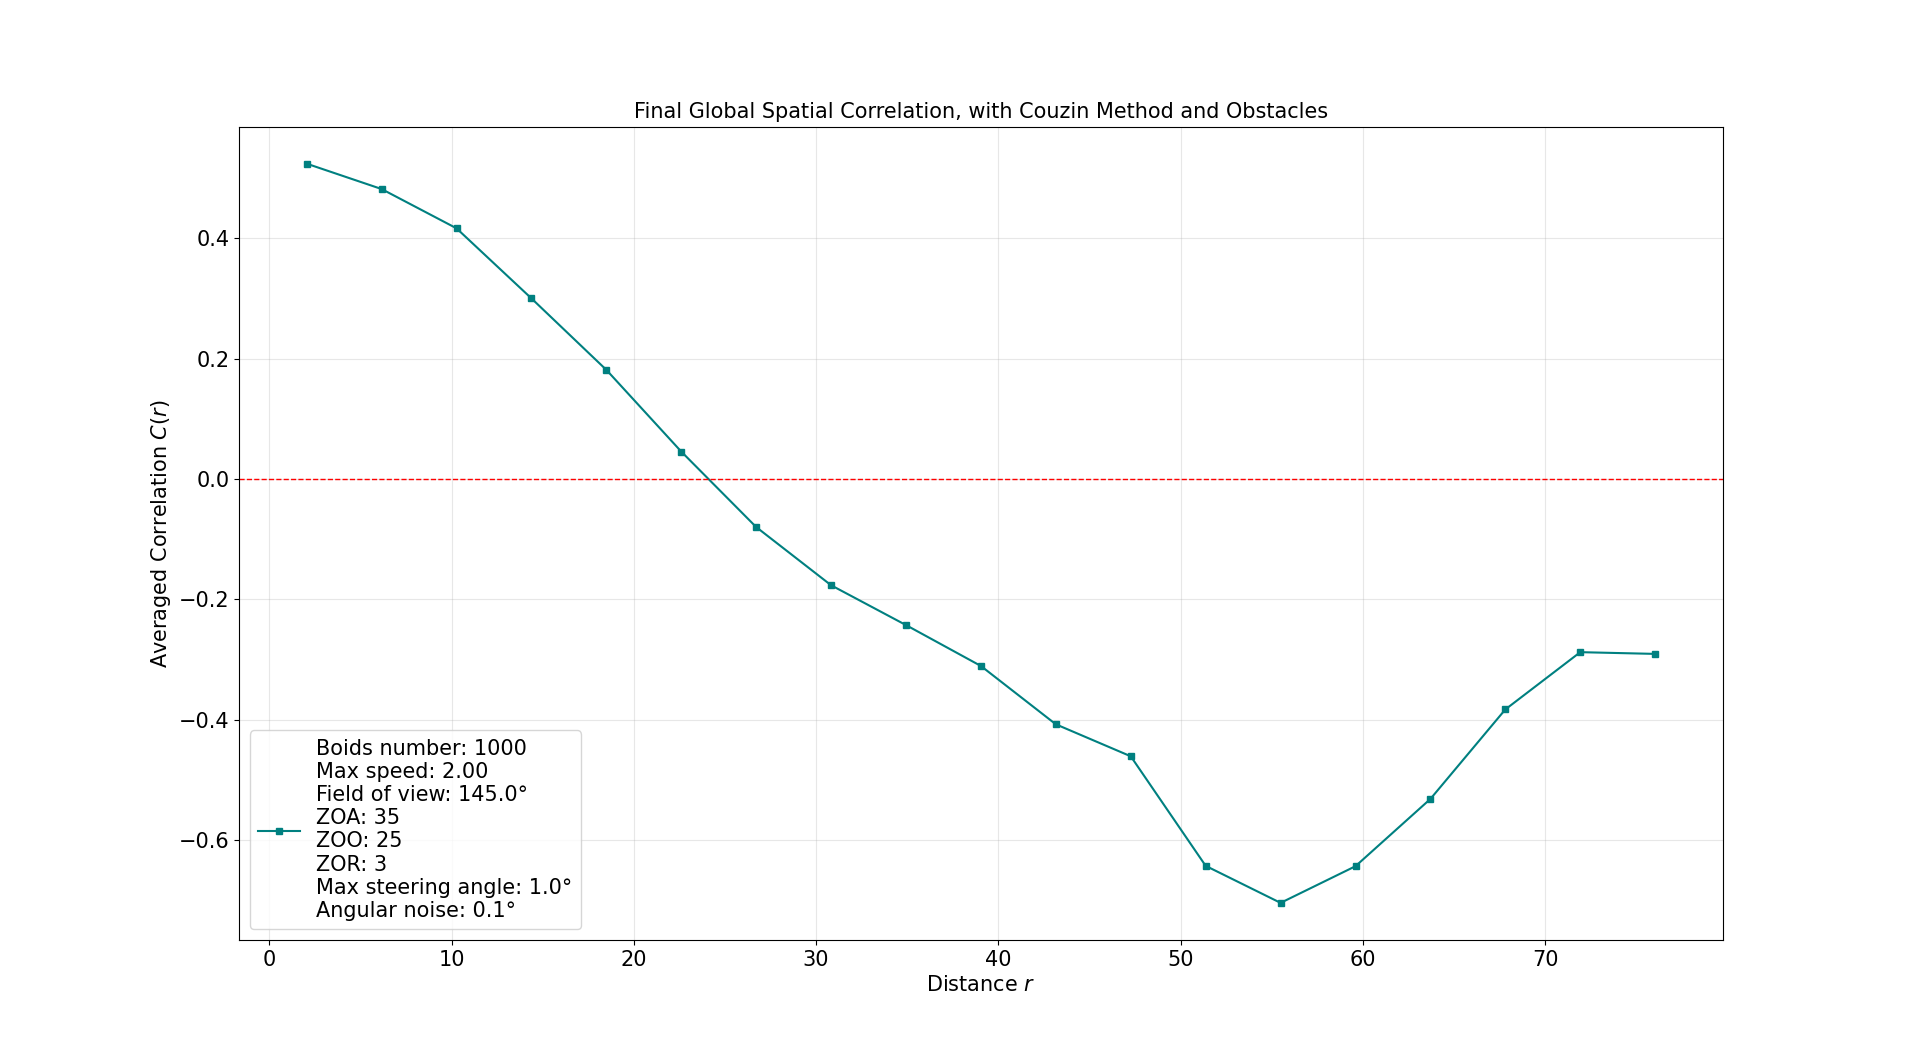
\includegraphics[width=\linewidth]{pictures/sec_4/couzin/1000_boids_couzin/column_cor_fun.png}
        \subcaption{Correlation function of a 1000 boids flock reacting to a column.}
    \end{subfigure}
    \begin{subfigure}{0.95\linewidth}
        
\includegraphics[width=\linewidth]{pictures/sec_4/couzin/500_boids_couzin/wall_cor_fun.png}
        \subcaption{Correlation function of a 500 boids flock reacting to a wall.}
    \end{subfigure}
    \caption{Correlation functions plotted in different situations for a flock simulated using Couzin's model.}
    \label{fig:couzin_cr}
\end{figure}
\subsubsection{Comments}
As expected, considering how Couzin's model is the most advanced one, it is the one that performs best, both quantitatively and qualitatively. That does come with a downside: the sensitivity to the parameters is comperable to Reynold's model, and as such the model requires its fair share of manual tuning in order for it to work as expected; nonetheless, the results are still the best across the tested methods, even when considering the time to manually tune the parameters.